\section{Respuestas a las Preguntas de Negocio Planteadas}
\label{sec:respuestas_preguntas}

En esta sección se presentan las tablas y visualizaciones generadas sobre el clúster de \textbf{Apache Spark} que dan respuesta cuantitativa a las preguntas de negocio formuladas en la Sección \ref{sec:preguntas_negocio}. Para garantizar la comparabilidad temporal entre criminalidad y accidentalidad, el análisis transversal se acota al primer semestre de 2026 (\texttt{2026-01-01} a \texttt{2026-06-30}), y cada hallazgo establece explícitamente su \textbf{punto de contacto con el entendimiento de negocio} descrito en la Sección \ref{sec:entendimiento_negocio}. (La Pregunta 8, por constituir el núcleo del modelado predictivo supervisado, se desarrolla y evalúa integralmente en la Sección \ref{sec:modelado_evaluacion}).

\subsection{Pregunta 1: Concentración Espacial y Temporal de Arrestos por Delitos Graves (Felonías) en los Condados de Nueva York}
\label{subsec:respuesta_q1}

\paragraph{Metodología y alcance:} Como se documentó en la valoración de restricciones (Sección \ref{sec:entendimiento_negocio}), el atributo \texttt{ARREST\_DATE} del conjunto \textit{NYPD Arrest Data} se publica con granularidad diaria (\texttt{MM/dd/yyyy}) sin marca de hora. En consecuencia, se analizó la distribución de los $55,651$ arrestos por delitos graves (\texttt{gravedad\_reportada = 'F'}, felonías) registrados entre enero y junio de 2026 a lo largo de los siete días de la semana y los cinco condados, calculando tanto el volumen absoluto como el peso porcentual intrasemanal dentro de cada condado (Tablas \ref{tab:q1_felonias_dia} y \ref{tab:q1_resumen_boro}, y Figura \ref{fig:q1_felonias_dia_boro}).

\begin{table}[H]
\centering
\scriptsize
\renewcommand{\arraystretch}{1.2}
\caption{Distribución de arrestos por delitos graves (Felonías, \texttt{F}) por día de la semana y condado (conteo y \% intrasemanal, 2026-I).}
\label{tab:q1_felonias_dia}
\begin{tabularx}{\linewidth}{l >{\raggedleft\arraybackslash}X >{\raggedleft\arraybackslash}X >{\raggedleft\arraybackslash}X >{\raggedleft\arraybackslash}X >{\raggedleft\arraybackslash}X >{\raggedleft\arraybackslash}X}
\toprule
\textbf{Día} & \textbf{BRONX} & \textbf{BROOKLYN} & \textbf{MANHATTAN} & \textbf{QUEENS} & \textbf{STATEN ISL.} & \textbf{TOTAL NYC} \\
\midrule
Lunes & 1,528 (11.81\%) & 2,132 (12.47\%) & 1,282 (10.59\%) & 1,401 (12.21\%) & 253 (12.44\%) & 6,596 (11.85\%) \\
Martes & \textbf{2,440 (18.85\%)} & 3,024 (17.69\%) & 2,059 (17.01\%) & 2,004 (17.47\%) & 354 (17.41\%) & 9,881 (17.76\%) \\
Miércoles & 2,431 (18.78\%) & \textbf{3,101 (18.14\%)} & 2,145 (17.72\%) & \textbf{2,161 (18.84\%)} & 352 (17.31\%) & \textbf{10,190 (18.31\%)} \\
Jueves & 2,068 (15.98\%) & 2,861 (16.73\%) & \textbf{2,213 (18.28\%)} & 1,959 (17.07\%) & \textbf{368 (18.10\%)} & 9,469 (17.01\%) \\
Viernes & 1,751 (13.53\%) & 2,414 (14.12\%) & 1,884 (15.56\%) & 1,587 (13.83\%) & 334 (16.43\%) & 7,970 (14.32\%) \\
Sábado & 1,388 (10.72\%) & 1,860 (10.88\%) & 1,377 (11.38\%) & 1,205 (10.50\%) & 183 (9.00\%) & 6,013 (10.80\%) \\
Domingo & 1,337 (10.33\%) & 1,705 (9.97\%) & 1,145 (9.46\%) & 1,156 (10.08\%) & 189 (9.30\%) & 5,532 (9.94\%) \\
\midrule
\textbf{Total} & \textbf{12,943 (100\%)} & \textbf{17,097 (100\%)} & \textbf{12,105 (100\%)} & \textbf{11,473 (100\%)} & \textbf{2,033 (100\%)} & \textbf{55,651 (100\%)} \\
\bottomrule
\end{tabularx}
\end{table}

\begin{table}[H]
\centering
\scriptsize
\renewcommand{\arraystretch}{1.2}
\caption{Indicadores de concentración intrasemanal de felonías por condado.}
\label{tab:q1_resumen_boro}
\resizebox{\textwidth}{!}{%
\begin{tabular}{l r c r r r}
\toprule
\textbf{Condado (\texttt{BORO})} & \textbf{Total felonías} & \textbf{Día pico} & \textbf{Arrestos día pico} & \textbf{Concentración Mar--Jue (\%)} & \textbf{Fin de semana Sáb--Dom (\%)} \\
\midrule
BROOKLYN & 17,097 & Miércoles & 3,101 & 52.56\% & 20.85\% \\
BRONX & 12,943 & Martes & 2,440 & \textbf{53.61\%} & 21.05\% \\
MANHATTAN & 12,105 & Jueves & 2,213 & 53.01\% & 20.84\% \\
QUEENS & 11,473 & Miércoles & 2,161 & 53.38\% & 20.58\% \\
STATEN ISLAND & 2,033 & Jueves & 368 & 52.82\% & 18.30\% \\
\bottomrule
\end{tabular}%
}
\end{table}

\begin{figure}[H]
    \centering
    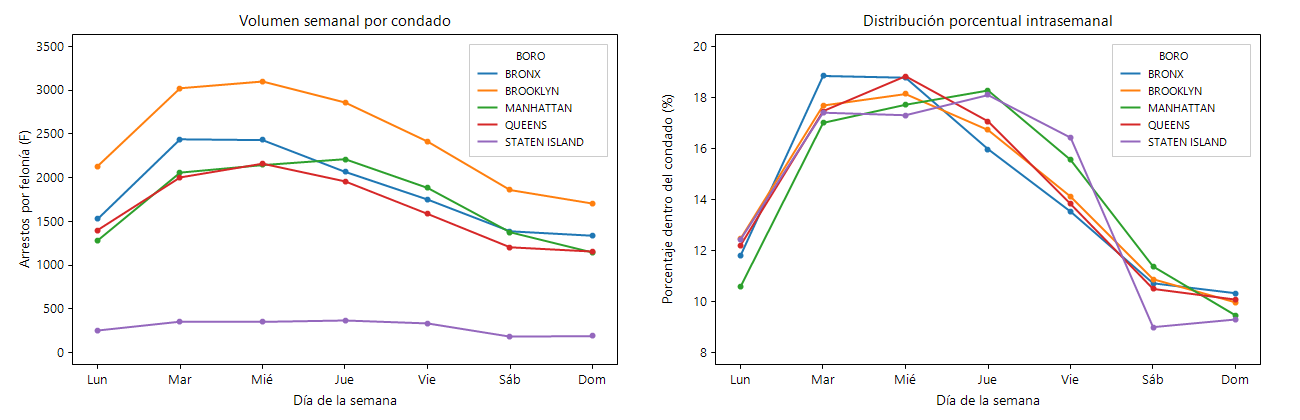
\includegraphics[width=0.96\textwidth]{imagenes/fig_q1_felonias_dia_boro.png}
    \caption{Volumen semanal absoluto (izquierda) y distribución porcentual intrasemanal (derecha) de arrestos por felonías (\texttt{F}) según condado.}
    \label{fig:q1_felonias_dia_boro}
\end{figure}

\paragraph{Interpretación y punto de contacto con el entendimiento de negocio:}
Brooklyn lidera el volumen absoluto de arrestos por delitos graves ($17,097$), seguido por el Bronx ($12,943$) y Manhattan ($12,105$). Sin embargo, al examinar el patrón porcentual intrasemanal (Figura \ref{fig:q1_felonias_dia_boro}, derecha), se descubre una regularidad operativa contundente: en los cinco condados, \textbf{entre el $52.56\%$ y el $53.61\%$ de todos los arrestos por felonías ocurren en tan solo tres días (martes, miércoles y jueves)}, sumando $29,540$ detenciones, mientras que los sábados y domingos apenas concentran el $20.75\%$ ($11,545$). Asimismo, se identifica un desplazamiento territorial del pico máximo: el Bronx alcanza su máximo los martes ($18.85\%$), Brooklyn y Queens los miércoles ($18.14\%$ y $18.84\%$), y Manhattan y Staten Island los jueves ($18.28\%$ y $18.10\%$). En conexión directa con el \textbf{Objetivo de Negocio 1 (\textit{NYPD CompStat})} de la Entrega 1, esta evidencia permite programar de manera escalonada los escuadrones especializados de cumplimiento de órdenes judiciales (\textit{warrant squads}) y refuerzos de patrulla: focalizando el Bronx los martes, Brooklyn y Queens los miércoles, y Manhattan los jueves.

\subsection{Pregunta 2: Correlación entre Pobreza Ponderada y Arrestos por Delitos Menores}
\label{subsec:respuesta_q2}

\paragraph{Metodología:} Se calculó la tasa de pobreza municipal ponderada de cada condado empleando el factor de expansión personal \texttt{PWGTP} sobre los registros válidos de \texttt{NYCgov\_Pov\_Stat} ($\in \{1, 2\}$), y se contrastó mediante el coeficiente de correlación lineal de Pearson ($r$) y su valor-$p$ bilateral frente a: (i) el conteo absoluto de arrestos por delitos menores (\texttt{gravedad\_reportada = 'M'}) en el primer semestre de 2026, y (ii) la tasa de arrestos por delitos menores por cada $100,000$ habitantes (Tabla \ref{tab:q2_pobreza_menores} y Figura \ref{fig:q2_pobreza_menores}).

\begin{table}[H]
\centering
\small
\renewcommand{\arraystretch}{1.2}
\caption{Tasa de pobreza ponderada (\texttt{PWGTP}) y arrestos por delitos menores (\texttt{M}) en volumen absoluto y tasa por 100,000 habitantes.}
\label{tab:q2_pobreza_menores}
\begin{tabular}{l r r r}
\toprule
\textbf{Condado (\texttt{BORO})} & \textbf{Pobreza ponderada (\%)} & \textbf{Arrestos menores (\texttt{M})} & \textbf{Menores por 100,000 hab.} \\
\midrule
BRONX & \textbf{27.12\%} & 19,268 & \textbf{1,388.12} \\
BROOKLYN & 20.31\% & \textbf{24,442} & 962.04 \\
QUEENS & 17.02\% & 16,767 & 744.95 \\
STATEN ISLAND & 16.00\% & 3,115 & 663.62 \\
MANHATTAN & 15.12\% & 19,337 & 1,243.81 \\
\bottomrule
\end{tabular}
\end{table}

\begin{figure}[H]
    \centering
    \begin{minipage}[c]{0.49\textwidth}
        \centering
        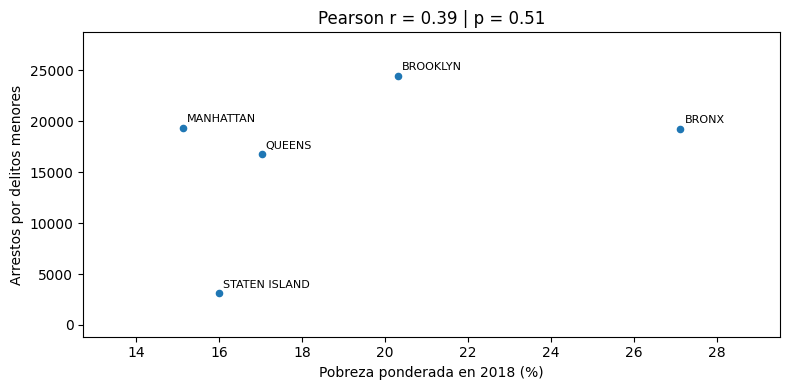
\includegraphics[width=\linewidth]{imagenes/fig_cell_51_1.png}
    \end{minipage}\hfill
    \begin{minipage}[c]{0.49\textwidth}
        \centering
        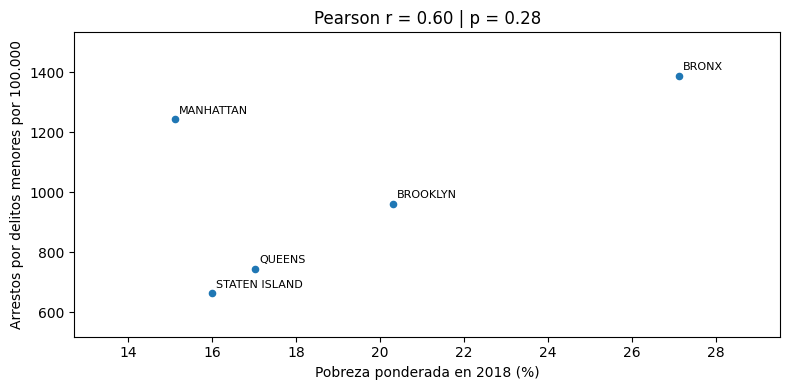
\includegraphics[width=\linewidth]{imagenes/fig_cell_51_2.png}
    \end{minipage}
    \caption{Diagramas de dispersión y correlación de Pearson entre pobreza ponderada (2018) y arrestos por delitos menores en conteo bruto (izquierda, $r=0.39$) y por 100,000 habitantes (derecha, $r=0.60$).}
    \label{fig:q2_pobreza_menores}
\end{figure}

\paragraph{Interpretación y punto de contacto con el entendimiento de negocio:}
Al comparar la pobreza ponderada con el conteo bruto de arrestos menores se obtiene una correlación débil de $r = 0.39$ ($p = 0.51$), debido a que Brooklyn domina por tamaño poblacional ($24,442$ casos) y Manhattan registra $19,337$ casos pese a tener la menor tasa de pobreza residente ($15.12\%$). Al corregir por población mediante la tasa por $100,000$ habitantes, la asociación positiva asciende a $r = 0.60$ ($p = 0.28$), ubicando al Bronx en el primer lugar tanto en pobreza ponderada ($27.12\%$) como en tasa de delitos menores ($1,388.12$ por $100,000$ hab.). Aunque con $n = 5$ condados el valor-$p$ no alcanza significancia estadística al $5\%$, el comportamiento confirma el diagnóstico macroeconómico planteado en la Sección \ref{sec:entendimiento_negocio} (\textbf{Objetivos 1 y 3}): en el Bronx la alta incidencia per cápita de contravenciones y delitos menores coincide con la vulnerabilidad económica estructural, mientras que en Manhattan ($1,243.81$ por $100,000$ hab. residentes) la tasa está inflada por el flujo diario de población flotante comercial y turística en el sistema de transporte y zonas comerciales.

\subsection{Pregunta 3: Factores Contribuyentes y Tipos de Vehículos en Colisiones con Peatones o Ciclistas Afectados}
\label{subsec:respuesta_q3}

\paragraph{Metodología:} Se filtraron las colisiones del primer semestre de 2026 con al menos un peatón o ciclista herido o fallecido. Para evitar subestimar causas o vehículos reportados en las posiciones secundarias, se inspeccionaron las cinco columnas de cada familia (\texttt{CONTRIBUTING FACTOR VEHICLE 1--5} y \texttt{VEHICLE TYPE CODE 1--5}), aplicando \texttt{array\_distinct} por \texttt{COLLISION\_ID} para contar una sola vez cada categoría presente en el siniestro y excluyendo valores genéricos (\texttt{UNSPECIFIED}, \texttt{UNKNOWN}, \texttt{DOES NOT APPLY} y \texttt{SIN\_VEHICULO\_*}) (Tabla \ref{tab:q3_vulnerables} y Figura \ref{fig:q3_vulnerables}).

\begin{table}[H]
\centering
\scriptsize
\renewcommand{\arraystretch}{1.2}
\caption{Top 10 de factores contribuyentes y tipos de vehículo en colisiones con peatones o ciclistas heridos/fallecidos (2026-I).}
\label{tab:q3_vulnerables}
\begin{tabularx}{\linewidth}{c X r c X r}
\toprule
\textbf{\#} & \textbf{Factor Contribuyente Reportado} & \textbf{Colisiones} & \textbf{\#} & \textbf{Tipo de Vehículo Reportado} & \textbf{Colisiones} \\
\midrule
1 & DRIVER INATTENTION/DISTRACTION & \textbf{1,686} & 1 & STATION WAGON/SPORT UTILITY VEHICLE & \textbf{1,741} \\
2 & FAILURE TO YIELD RIGHT-OF-WAY & \textbf{1,243} & 2 & SEDAN & \textbf{1,554} \\
3 & PEDESTRIAN/BICYCLIST ERROR/CONFUSION & 378 & 3 & BICYCLIST & 1,035 \\
4 & TRAFFIC CONTROL DISREGARDED & 170 & 4 & BIKE & 982 \\
5 & BACKING UNSAFELY & 144 & 5 & 4 DR SEDAN & 762 \\
6 & UNSAFE SPEED & 140 & 6 & TAXI & 242 \\
7 & PASSING OR LANE USAGE IMPROPER & 135 & 7 & PICK-UP TRUCK & 162 \\
8 & TURNING IMPROPERLY & 115 & 8 & VAN & 106 \\
9 & VIEW OBSTRUCTED/LIMITED & 99 & 9 & BUS & 83 \\
10 & OTHER VEHICULAR & 98 & 10 & MOPED & 74 \\
\bottomrule
\end{tabularx}
\end{table}

\begin{figure}[H]
    \centering
    \begin{minipage}[c]{0.49\textwidth}
        \centering
        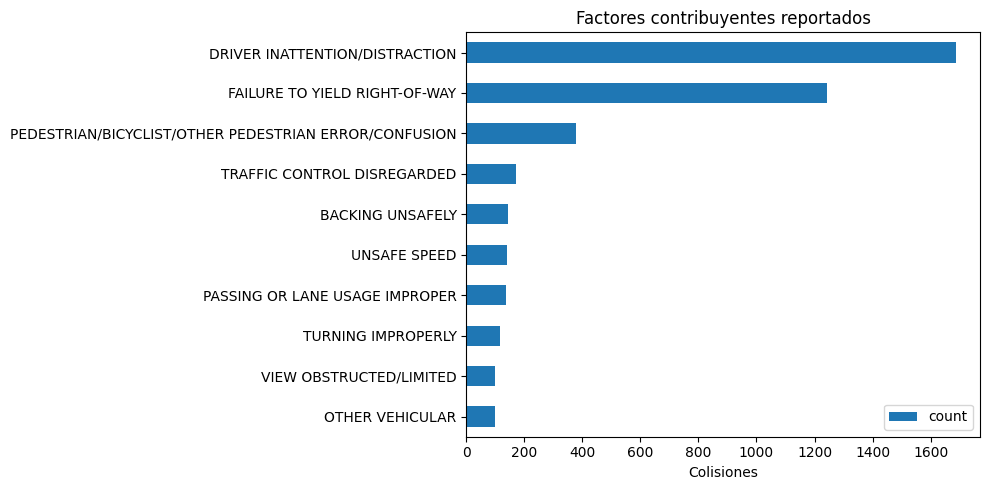
\includegraphics[width=\linewidth]{imagenes/fig_cell_54_1.png}
    \end{minipage}\hfill
    \begin{minipage}[c]{0.49\textwidth}
        \centering
        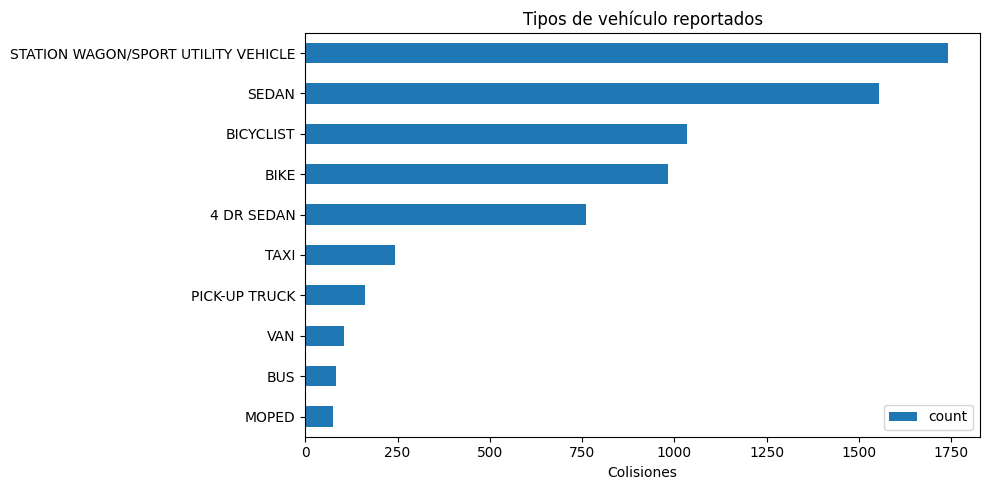
\includegraphics[width=\linewidth]{imagenes/fig_cell_54_2.png}
    \end{minipage}
    \caption{Principales factores contribuyentes (izquierda) y tipos de vehículo (derecha) en siniestros con afectación de peatones o ciclistas.}
    \label{fig:q3_vulnerables}
\end{figure}

\paragraph{Interpretación y punto de contacto con el entendimiento de negocio:}
Dos factores humanos del conductor concentran por amplio margen la accidentalidad contra actores viales vulnerables: la \textbf{distracción o falta de atención del conductor (\texttt{DRIVER INATTENTION/DISTRACTION}, $1,686$ colisiones)} y el \textbf{no ceder la prelación de paso (\texttt{FAILURE TO YIELD RIGHT-OF-WAY}, $1,243$ colisiones)}, seguidos a gran distancia por error/confusión del peatón o ciclista ($378$), desacato de señales de tránsito ($170$), reversa insegura ($144$) y velocidad insegura ($140$). En cuanto al parque automotor, las \textbf{camionetas familiares y SUV (\texttt{STATION WAGON/SPORT UTILITY VEHICLE}, $1,741$ colisiones)} encabezan los siniestros con vulnerables, superando incluso a los sedanes ($1,554$). Esto se conecta directamente con el \textbf{Objetivo de Negocio 2 (\textit{NYC DOT Vision Zero})} de la Entrega 1: la mayor altura del capó y los puntos ciegos de las SUV incrementan la severidad de los atropellamientos en giros, por lo que el NYC DOT debe priorizar fases semafóricas exclusivas para peatones (\textit{Leading Pedestrian Intervals}, LPI) e isletas de refugio en intersecciones para mitigar directamente el factor \texttt{FAILURE TO YIELD RIGHT-OF-WAY}.

\subsection{Pregunta 4: Desempleo, Nivel Educativo y Siniestralidad Vial Fatal por Condado}
\label{subsec:respuesta_q4}

\paragraph{Metodología:} Se estimó la tasa ponderada de desempleo en la fuerza laboral civil ($\texttt{ESR} = 3$ sobre $\texttt{ESR} \in \{1, 2, 3\}$) y la distribución porcentual del nivel educativo alcanzado en adultos de $25$ años o más ($\texttt{SCHL} \in [1, 24]$) usando \texttt{PWGTP}. Estos indicadores se cruzaron con el conteo y la tasa de colisiones fatales (al menos un fallecido) por cada $100,000$ habitantes en el primer semestre de 2026 (Tabla \ref{tab:q4_desempleo_edu_fatal} y Figura \ref{fig:q4_desempleo_edu_fatal}).

\begin{table}[H]
\centering
\scriptsize
\renewcommand{\arraystretch}{1.2}
\caption{Indicadores laborales y educativos (ponderados con \texttt{PWGTP}) frente a la tasa de colisiones fatales por 100,000 habitantes (2026-I).}
\label{tab:q4_desempleo_edu_fatal}
\resizebox{\textwidth}{!}{%
\begin{tabular}{l r r r r r r r}
\toprule
\textbf{Condado} & \textbf{Desempleo (\%)} & \textbf{Sin sec. (\%)} & \textbf{Secundaria (\%)} & \textbf{Sup. sin grado (\%)} & \textbf{Univ. o sup. (\%)} & \textbf{Fatales} & \textbf{Fatales / 100k} \\
\midrule
QUEENS & 5.11\% & 17.32\% & 26.53\% & 22.29\% & 33.87\% & \textbf{31} & \textbf{1.38} \\
BRONX & \textbf{9.56\%} & \textbf{26.26\%} & 27.34\% & 25.15\% & 21.25\% & 19 & 1.37 \\
MANHATTAN & 4.36\% & 11.80\% & 12.43\% & 13.35\% & \textbf{62.41\%} & 21 & 1.35 \\
BROOKLYN & 4.67\% & 16.42\% & 24.94\% & 19.09\% & 39.55\% & 26 & 1.02 \\
STATEN ISLAND & 4.40\% & 12.17\% & \textbf{30.91\%} & 23.61\% & 33.31\% & 3 & 0.64 \\
\bottomrule
\end{tabular}%
}
\end{table}

\begin{figure}[H]
    \centering
    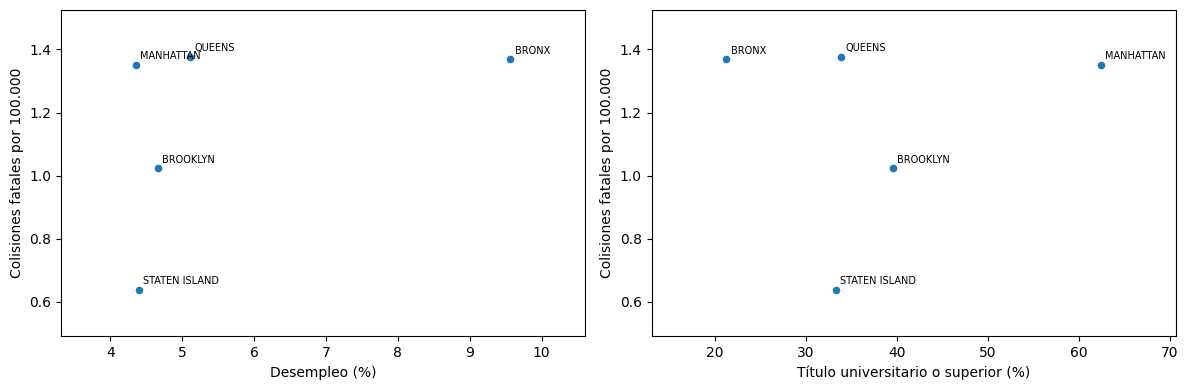
\includegraphics[width=0.95\textwidth]{imagenes/fig_cell_57_1.png}
    \caption{Tasa de colisiones fatales por 100,000 habitantes frente a la tasa de desempleo (izquierda) y al porcentaje de población con título universitario o superior (derecha).}
    \label{fig:q4_desempleo_edu_fatal}
\end{figure}

\paragraph{Interpretación y punto de contacto con el entendimiento de negocio:}
Los resultados revelan que la mortalidad vial por cada $100,000$ habitantes es prácticamente idéntica en tres condados con perfiles socioeconómicos opuestos: \textbf{Queens ($1.38$), el Bronx ($1.37$) y Manhattan ($1.35$)}, pese a que el Bronx duplica la tasa de desempleo de Manhattan ($9.56\%$ frente a $4.36\%$) y Manhattan casi triplica la proporción de graduados universitarios del Bronx ($62.41\%$ frente a $21.25\%$). Esto responde directamente a la hipótesis planteada en los \textbf{Objetivos 2 y 3} del entendimiento de negocio: a escala agregada de condado, la letalidad vial no está determinada de forma lineal simple por el nivel educativo o el desempleo promedio del condado, sino por la combinación de déficit de infraestructura segura en corredores de carga (como en el Bronx y Queens) y la altísima densidad de interacciones peatonales en centros comerciales (Manhattan), lo que exige descender a una escala microterritorial de cuadrículas como se realiza en la Pregunta 5 y en el modelo K-Means.

\subsection{Pregunta 5: Las Cinco ``Zonas Calientes Duales'' (\textit{Hotspots}) de Arrestos y Colisiones Fatales}
\label{subsec:respuesta_q5}

\paragraph{Metodología:} Se discretizaron los registros con coordenadas válidas del primer semestre de 2026 en celdas uniformes de $0.01^\circ \times 0.01^\circ$ ($\approx 1.1\text{ km} \times 0.85\text{ km}$). Sobre las celdas que registraron simultáneamente arrestos y colisiones fatales, se construyó un índice compuesto promediando el rango percentil (\texttt{percent\_rank}) del volumen de arrestos y el rango percentil de colisiones fatales:
\[
\text{Índice}_{x,y} = \frac{1}{2}\Big[\text{PercentRank}(\text{arrestos}_{x,y}) + \text{PercentRank}(\text{fatales}_{x,y})\Big].
\]
La Tabla \ref{tab:q5_hotspots} y la Figura \ref{fig:q5_hotspots} presentan las cinco cuadrículas críticas que encabezan el ranking de la ciudad.

\begin{table}[H]
\centering
\scriptsize
\renewcommand{\arraystretch}{1.2}
\caption{Top 5 de cuadrículas urbanas ($0.01^\circ \times 0.01^\circ$) con mayor concentración conjunta de arrestos y colisiones fatales (2026-I).}
\label{tab:q5_hotspots}
\resizebox{\textwidth}{!}{%
\begin{tabular}{c r r l r r r}
\toprule
\textbf{Puesto} & \textbf{Latitud centro} & \textbf{Longitud centro} & \textbf{Sector urbano de referencia} & \textbf{Arrestos} & \textbf{Colisiones fatales} & \textbf{Índice conjunto} \\
\midrule
1 & $40.845^\circ$ & $-73.905^\circ$ & Bronx Central (\textit{Tremont / Cross Bronx Expwy}) & \textbf{1,584} & \textbf{2} & \textbf{0.9674} \\
2 & $40.675^\circ$ & $-73.905^\circ$ & Brooklyn Este (\textit{Brownsville / Broadway Jct}) & \textbf{1,107} & \textbf{2} & \textbf{0.9511} \\
3 & $40.755^\circ$ & $-73.965^\circ$ & Manhattan Midtown East (\textit{2nd/3rd Ave \& E 50s}) & 138 & \textbf{2} & 0.7554 \\
4 & $40.635^\circ$ & $-74.135^\circ$ & Staten Island North Shore (\textit{Port Richmond}) & 109 & \textbf{2} & 0.7228 \\
5 & $40.715^\circ$ & $-73.975^\circ$ & Manhattan Lower East Side (\textit{Williamsburg Br / FDR}) & 77 & \textbf{2} & 0.6902 \\
\bottomrule
\end{tabular}%
}
\end{table}

\begin{figure}[H]
    \centering
    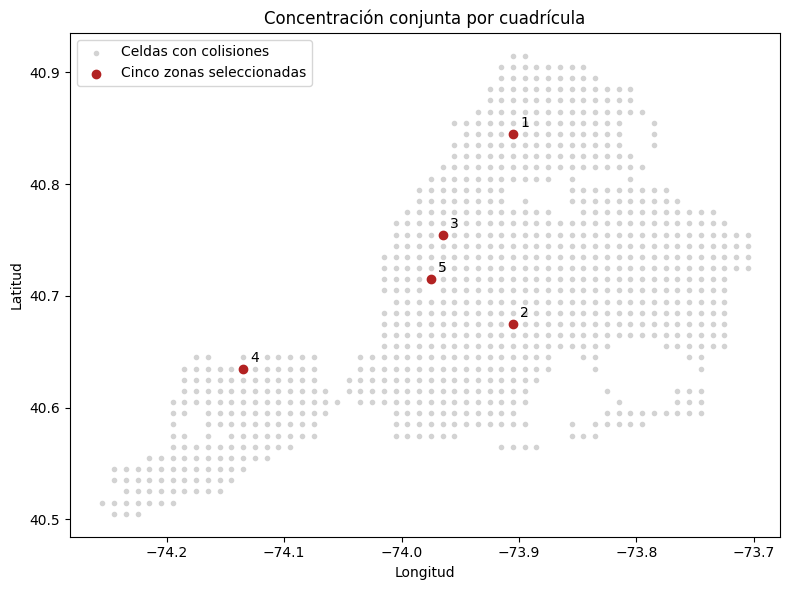
\includegraphics[width=0.72\textwidth]{imagenes/fig_cell_60_1.png}
    \caption{Mapa de cuadrículas activas con colisiones en NYC y localización exacta de las 5 zonas calientes duales seleccionadas.}
    \label{fig:q5_hotspots}
\end{figure}

\paragraph{Interpretación y punto de contacto con el entendimiento de negocio:}
Las dos primeras zonas calientes duales sobresalen de manera extraordinaria: la cuadrícula centrada en $(40.845^\circ, -73.905^\circ)$ en el corredor central del Bronx (\textit{Tremont / Cross Bronx Expressway}, área de los precintos 44, 46 y 48) acumula \textbf{$1,584$ arrestos y $2$ colisiones mortales} ($\text{índice} = 0.9674$), seguida por la cuadrícula $(40.675^\circ, -73.905^\circ)$ en el este de Brooklyn (\textit{Brownsville / Broadway Junction}, área de los precintos 73 y 75, que encabezaban el Elemento 7 del EDA) con \textbf{$1,107$ arrestos y $2$ colisiones mortales} ($\text{índice} = 0.9511$). Este resultado materializa el criterio de éxito central de la Sección \ref{sec:entendimiento_negocio}: entrega a la Alcaldía de Nueva York cinco coordenadas precisas de menos de $1\text{ km}^2$ donde la inversión simultánea en iluminación peatonal, rediseño de cruces arteriales y presencia policial genera un impacto directo tanto en \textit{CompStat} como en \textit{Vision Zero}.

\subsection{Pregunta 6: Perfil Demográfico de los Arrestos según Nivel de Gravedad de la Ofensa}
\label{subsec:respuesta_q6}

\paragraph{Metodología:} Utilizando funciones de ventana particionadas por la gravedad original reportada (\texttt{V}, \texttt{M}, \texttt{F}), se identificó el perfil demográfico conjunto más frecuente (\texttt{AGE\_GROUP}, \texttt{PERP\_SEX}, \texttt{PERP\_RACE}) y se graficó la composición porcentual separada de cada variable demográfica por categoría de gravedad (Tabla \ref{tab:q6_perfil_demografico} y Figura \ref{fig:q6_perfil_demografico}).

\begin{table}[H]
\centering
\scriptsize
\renewcommand{\arraystretch}{1.2}
\caption{Perfil demográfico conjunto modal según el nivel de gravedad reportado de la ofensa (2026-I).}
\label{tab:q6_perfil_demografico}
\resizebox{\textwidth}{!}{%
\begin{tabular}{c l c c l r}
\toprule
\textbf{Código} & \textbf{Nivel de gravedad} & \textbf{Grupo etario modal} & \textbf{Sexo modal} & \textbf{Raza registrada modal} & \textbf{Arrestos del perfil modal} \\
\midrule
\texttt{F} & Felonía (\textit{Felony}) & \texttt{25-44} & \texttt{M} (Masculino) & \texttt{BLACK} & 12,539 \\
\texttt{M} & Delito menor (\textit{Misdemeanor}) & \texttt{25-44} & \texttt{M} (Masculino) & \texttt{BLACK} & 17,778 \\
\texttt{V} & Contravención (\textit{Violation}) & \texttt{25-44} & \texttt{M} (Masculino) & \texttt{BLACK} & 570 \\
\bottomrule
\end{tabular}%
}
\end{table}

\begin{figure}[H]
    \centering
    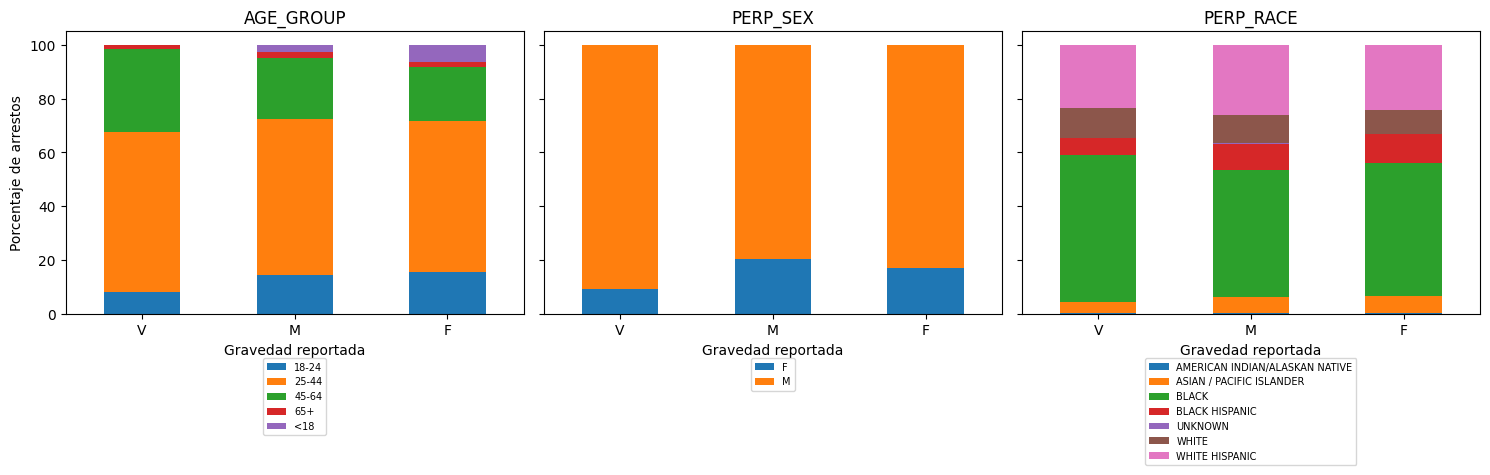
\includegraphics[width=0.98\textwidth]{imagenes/fig_cell_63_1.png}
    \caption{Composición porcentual de los arrestos según gravedad reportada (\texttt{V}, \texttt{M}, \texttt{F}) desagregada por grupo etario, sexo y raza.}
    \label{fig:q6_perfil_demografico}
\end{figure}

\paragraph{Interpretación y punto de contacto con el entendimiento de negocio:}
En las tres categorías penales (\texttt{V}, \texttt{M} y \texttt{F}), el grupo modal invariante corresponde a hombres de $25$ a $44$ años registrados como \texttt{BLACK} ($17,778$ en delitos menores, $12,539$ en felonías y $570$ en contravenciones). Asimismo, la Figura \ref{fig:q6_perfil_demografico} muestra que la proporción de jóvenes de \texttt{18-24} años y menores de $18$ años (\texttt{<18}) es mayor en las felonías (\texttt{F}) que en los delitos menores (\texttt{M}). En línea con los \textbf{Objetivos 1 y 3} del entendimiento de negocio, es fundamental subrayar que estas cifras reflejan la composición de las detenciones policiales registradas y deben articularse con programas de inserción laboral juvenil y prevención social comunitaria de \textit{NYC Opportunity} en los distritos de mayor vulnerabilidad.

\subsection{Pregunta 7: Comportamiento Horario de las Colisiones en Manhattan frente a Staten Island}
\label{subsec:respuesta_q7}

\paragraph{Metodología:} Se compararon las colisiones con hora válida del primer semestre de 2026 entre Manhattan (condado de altísima densidad comercial y población flotante) y Staten Island (condado residencial y suburbano), analizando tanto la frecuencia horaria absoluta como la curva porcentual normalizada dentro de cada condado para aislar la forma del patrón intradiario respecto del tamaño total (Tabla \ref{tab:q7_horario_manhattan_si} y Figura \ref{fig:q7_horario_manhattan_si}).

\begin{table}[H]
\centering
\scriptsize
\renewcommand{\arraystretch}{1.2}
\caption{Resumen comparativo del régimen horario de colisiones entre Manhattan y Staten Island (2026-I).}
\label{tab:q7_horario_manhattan_si}
\resizebox{\textwidth}{!}{%
\begin{tabular}{l r c r r}
\toprule
\textbf{Condado (\texttt{BOROUGH})} & \textbf{Total colisiones (2026-I)} & \textbf{Hora pico} & \textbf{Colisiones en hora pico} & \textbf{\% en hora pico dentro del condado} \\
\midrule
MANHATTAN & \textbf{7,347} & \textbf{16:00 h} & \textbf{507} & 6.90\% \\
STATEN ISLAND & 1,570 & \textbf{15:00 h} & 112 & \textbf{7.13\%} \\
\bottomrule
\end{tabular}%
}
\end{table}

\begin{figure}[H]
    \centering
    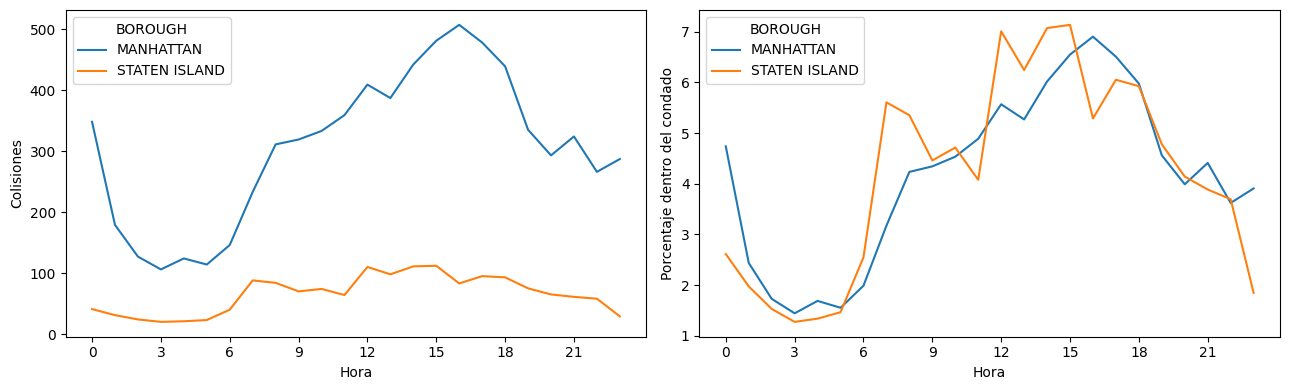
\includegraphics[width=0.96\textwidth]{imagenes/fig_cell_66_1.png}
    \caption{Comparación del volumen horario absoluto (izquierda) y del porcentaje intradiario dentro de cada condado (derecha) de las colisiones en Manhattan y Staten Island.}
    \label{fig:q7_horario_manhattan_si}
\end{figure}

\paragraph{Interpretación y punto de contacto con el entendimiento de negocio:}
Manhattan registra un volumen $4.68$ veces superior al de Staten Island ($7,347$ frente a $1,570$ colisiones). Sin embargo, la gráfica de proporciones internas (Figura \ref{fig:q7_horario_manhattan_si}, derecha) revela dos dinámicas urbanas estructuralmente distintas que validan la hipótesis del \textit{``Efecto Manhattan''} formulada en el entendimiento de negocio (\textbf{Objetivo 2 --- NYC DOT}):
\begin{enumerate}
    \item \textbf{En Staten Island (patrón bimodal pendular escolar--laboral):} Se observan dos picos agudos en horas de desplazamiento residencial: un pico matutino entre las \textbf{07:00 y las 08:00 h} ($\sim 5.6\%$ por hora) y un pico vespertino temprano entre las \textbf{12:00 y las 15:00 h} (máximo a las \textbf{15:00 h} con $112$ choques, $7.13\%$, coincidente con la salida escolar y laboral suburbana), cayendo abruptamente en la noche y la madrugada ($<2\%$ a las 23:00--05:00 h).
    \item \textbf{En Manhattan (meseta comercial continua y actividad nocturna):} El ascenso matutino es más gradual, sostiene una meseta alta durante toda la jornada laboral y comercial con máximo a las \textbf{16:00 h} ($507$ colisiones, $6.90\%$), y mantiene una proporción significativamente superior durante la noche y la madrugada (\textbf{21:00 a 01:00 h}, con casi el $4.8\%$ a las 00:00 h frente al $2.6\%$ en Staten Island), impulsada por la vida nocturna, taxis y logística urbana. Esto justifica planes de semaforización adaptativa y control nocturno diferenciados por condado.
\end{enumerate}
